
\documentclass{Setup/template_isec_class}

% Template ISEC/LaTeX, janeiro 2023
%--------------------------------------
\usepackage{Setup/template_isec_package}
%--------------------------------------

%--------------------------------------
% Obs#1
% Onde incluir todos os ficheiros (package)
% e instruções adicionais para este projeto
\usepackage{extras}
%--------------------------------------

\begin{document}

%--------------------------------------
% Obs#2
% Definir qual o título e quais os autores do trabalho
\newcommand{\titulotrabalho}{Métodos Numéricos para EDO/PVI}
\newcommand{\autorestrabalho}{António Pedroso, António Rocha, Samuel Costa}
%--------------------------------------

\pagestyle{empty}

% Capa
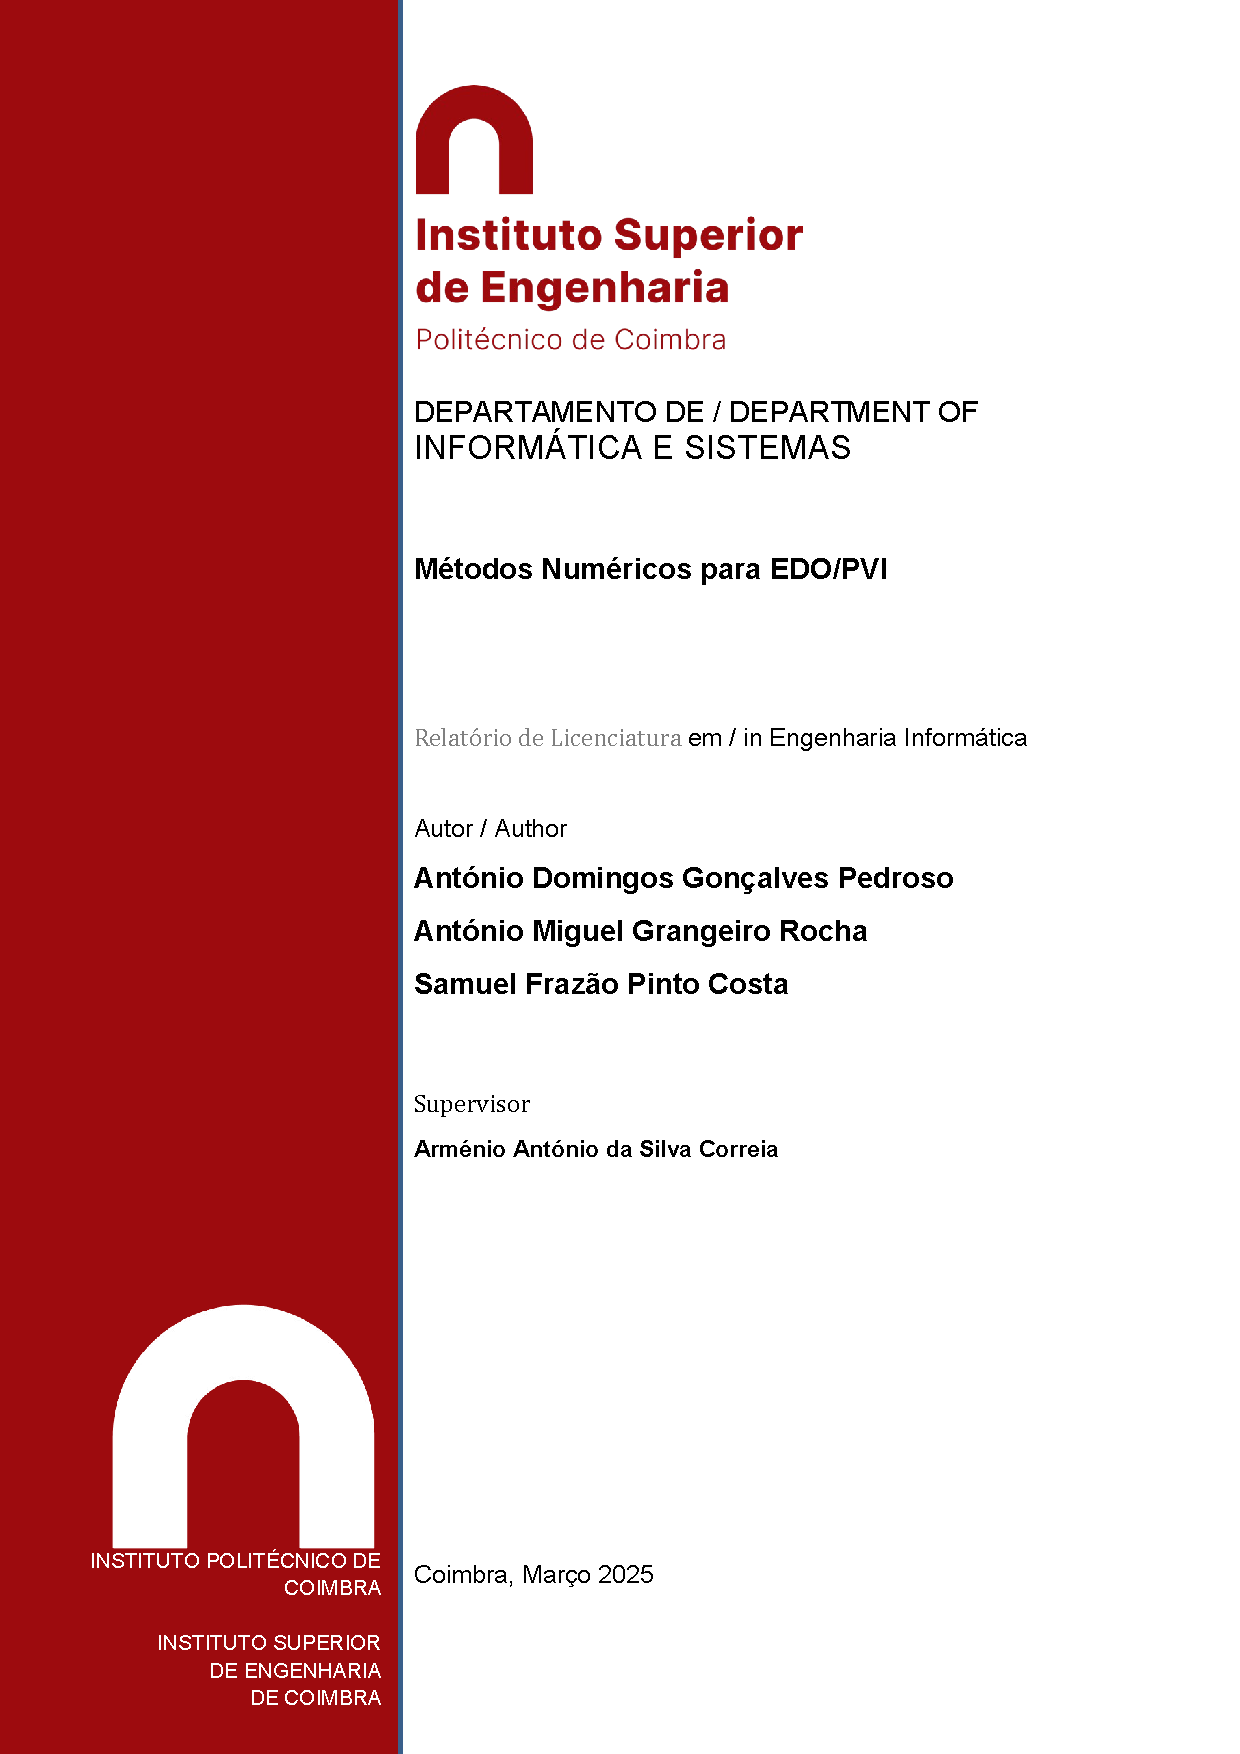
\includepdf{Inicio/capa}

\newpage

%--------------------------------------
\pagestyle{fancy}
\fancyhf{}
\fancyhead{}
\fancyhead[CO]{\nouppercase{\truncate{\headwidth}{\titulotrabalho}}}
\fancyhead[CE]{\nouppercase{\autorestrabalho}}
\renewcommand{\headrulewidth}{0pt}
\fancyfoot{}
\fancyfoot[CO,CE]{\thepage}
\setlength{\headheight}{14.5pt}
\fancypagestyle{plain}{}
%--------------------------------------

\pagenumbering{roman}

% Resumo PT
\phantomsection
\addcontentsline{toc}{chapter}{Resumo}

% Resumo
%--------------------------------------
\vspace*{45pt}
\begin{flushleft}
	{\Large \textbf{\scshape{Resumo}}}
\end{flushleft}
\vspace*{10pt}

\begin{resumo}
Este relatório documenta o desenvolvimento da Atividade 3 da unidade curricular de Análise Matemática 2, centrada nos métodos numéricos para a resolução de Equações Diferenciais Ordinárias (EDO). São abordados diversos métodos, nomeadamente o método de Euler, o método de Euler melhorado (Heun), e os métodos de Runge-Kutta de ordem 2, 3 e 4, bem como o solver \texttt{ode45} do \textsc{Matlab}. Para cada método, é apresentada a respetiva formulação matemática, juntamente com uma análise comparativa da sua eficácia, precisão e aplicabilidade. A atividade permitiu consolidar conhecimentos teóricos e práticos na resolução numérica de EDOs, demonstrando a importância destas ferramentas em contextos de modelação matemática e simulação computacional.
\end{resumo}

\newpage

% Abstract ENG
\phantomsection
\addcontentsline{toc}{chapter}{Abstract}

% Abstract
%--------------------------------------
\vspace*{45pt}
\begin{flushleft}
	{\Large \textbf{\scshape{Abstract}}}
\end{flushleft}
\vspace*{10pt}

\begin{abstract}
This report documents the development of Activity 3 from the course unit Mathematical Analysis 2, focused on numerical methods for solving Ordinary Differential Equations (ODEs). Several methods are addressed, including Euler’s method, the improved Euler method (Heun), and the Runge-Kutta methods of order 2, 3, and 4, as well as the \texttt{ode45} solver from \textsc{Matlab}. Each method is presented with its corresponding mathematical formulation and a comparative analysis regarding its effectiveness, accuracy, and applicability. This activity allowed for the consolidation of both theoretical and practical knowledge in the numerical resolution of ODEs, highlighting the importance of these tools in mathematical modeling and computational simulation.
\end{abstract}


\newpage

% Epígrafe
\phantomsection
\addcontentsline{toc}{chapter}{Ep\'{\i}grafe}

% Epígrafe
%--------------------------------------
\vspace*{45pt}
\begin{flushleft}
	{\Large \textbf{\scshape{Ep\'{\i}grafe}}}
\end{flushleft}
\vspace*{10pt}

\begin{flushright}
	Tzzzzz Tzzzzzzz Tzzzzzz. \\
	Arménio, 2025
\end{flushright}



\newpage

% Dedicatória
%\phantomsection
%\addcontentsline{toc}{chapter}{Dedicat\'{o}ria}
%
% Dedicatória
%--------------------------------------
\vspace*{45pt}
\begin{flushleft}
	{\Large \textbf{\scshape{Dedicat\'{o}ria}}}
\end{flushleft}
\vspace*{10pt}


Goat armenio


%\newpage

% Agradecimentos
\phantomsection
\addcontentsline{toc}{chapter}{Agradecimentos}

% Agradecimentos
%--------------------------------------
\vspace*{45pt}
\begin{flushleft}
	{\Large \textbf{\scshape{Agradecimentos}}}
\end{flushleft}
\vspace*{10pt}


Arménio António da Silva Correia

Rui Manuel Carreira Rodrigues

\newpage



\renewcommand{\contentsname}{\'{I}ndice}
\renewcommand{\listtablename}{\'{I}ndice de tabelas}
\renewcommand{\listfigurename}{\'{I}ndice de figuras}

\phantomsection
\addcontentsline{toc}{chapter}{\'{I}ndice}
\tableofcontents

%\newpage

%\phantomsection
%\addcontentsline{toc}{chapter}{\'{I}ndice de tabelas}
%\listoftables

\newpage

\phantomsection
\addcontentsline{toc}{chapter}{\'{I}ndice de figuras}
\listoffigures

\newpage

% Lista de abreviaturas
\phantomsection
\addcontentsline{toc}{chapter}{Lista de abreviaturas}

% Lista de abreviaturas
%--------------------------------------
\vspace*{45pt}
\begin{flushleft}
	{\Large \textbf{\scshape{Lista de abreviaturas}}}
\end{flushleft}
\vspace*{20pt}

\begin{tabular}{l l}
EDO     & Equação Diferencial Ordinária \\
IEEE	& \textit{Institute of Electrical and Electronics Engineers} \\
ISEC    & Instituto Superior de Engenharia de Coimbra \\
k1, k2, k3, k4 & Avaliações intermediárias da função diferencial \\
MATLAB  & \textit{Matrix Laboratory} \\
ODE     & \textit{Ordinary Differential Equation} \\
PVI     & Problema de Valor Inicial \\
RK2     & Método de Runge-Kutta de Ordem 2 \\
RK3     & Método de Runge-Kutta de Ordem 3 \\
RK4     & Método de Runge-Kutta de Ordem 4 \\
RK45    & Método de Runge-Kutta de Ordem 4(5), usado pelo \texttt{ode45} \\
\texttt{ode45} & Função do MATLAB para resolver EDOs com método adaptativo \\
$t$      & Variável independente (tempo) \\
$y$      & Variável dependente (solução da EDO) \\
$y_0$    & Condição inicial da variável dependente \\
$h$      & Tamanho do passo (step size) \\
$a$      & Limite inferior do intervalo \\
$b$      & Limite superior do intervalo \\
$f(t, y)$ & Função que define a EDO, ou seja, $y' = f(t, y)$ \\
\end{tabular}


%\newpage

% Lista de símbolos
%\phantomsection
%\addcontentsline{toc}{chapter}{Lista de s\'{\i}mbolos}
%
% Lista de símbolos
%--------------------------------------
\vspace*{45pt}
\begin{flushleft}
	{\Large \textbf{\scshape{Lista de símbolos}}}
\end{flushleft}
\vspace*{20pt}

\begin{tabular}{l l}
    $\mathrm{kN}$       &   Quilonewton\\
    $\varepsilon_{ax}$  &   Extensão axial (\%)\\
    % deve acrescentar aqui os símbolos que considerar necessários, por ordem alfabética    
\end{tabular}



\newpage
\pagenumbering{arabic}

% Capítulo inicial
% Introdução

% Introdução
%--------------------------------------
\chapter{Introdução}


No presente documento, será registado todo o processo envolvido na realização da Atividade 3: Métodos Numéricos para EDO/PVI, proposta no âmbito da Unidade Curricular Análise Matemática 2.

Os assuntos abordados neste relatório baseiam-se, principalmente, nos conhecimentos transmitidos nas aulas, sendo ainda complementados com pesquisa e trabalho realizado fora do ambiente letivo.

Ao longo deste documento, será possível acompanhar todo o trabalho desenvolvido nesta atividade, as dificuldades enfrentadas e a descrição detalhada de todas as suas componentes.



% NEuler

% EDO
%--------------------------------------
\chapter{Equações Diferenciais Ordinárias (EDO)}

O estudo de Equações Diferenciais Ordinárias (EDO) foca-se na resolução de equações da forma:

\begin{equation}
\begin{cases}
x'(t) = f(t, x(t)) \\
x(t_0) = x_0
\end{cases}
\end{equation}

em que $x$ e $f$ podem ser funções escalares ou vetoriais. O objetivo é determinar a função $x(t)$ para $t > t_0$, conhecendo-se o valor inicial $x_0$ no instante $t_0$. Estas equações surgem frequentemente na modelação de fenómenos físicos, biológicos, económicos, entre outros.

Na prática, a solução analítica destas equações nem sempre é possível, pelo que se recorre a métodos numéricos para obter aproximações da solução.

% NEuler
% Método de Euler
%--------------------------------------
\chapter{Método de Euler}

\section*{3.1 Fórmulas}

O método de Euler é um procedimento numérico de primeira ordem ($y'$) para aproximar a solução da equação diferencial que satisfaz a condição inicial:

\begin{equation}
y' = f(t, y)
\end{equation}

\begin{equation}
y(t_0) = y_0
\end{equation}

O Método de Euler para resolver um Problema de Valor Inicial (PVI) é dado pela seguinte fórmula geral:

\begin{equation}
y_{i+1} = y_i + h f(t_i, y_i)
\end{equation}

onde:
\begin{itemize}
    \item $y_{i+1}$ → Próximo valor aproximado da solução do problema original (na abscissa $t_{i+1}$);
    \item $y_i$ → Valor aproximado da solução do problema original na abscissa atual;
    \item $h$ → Valor de cada subintervalo (passo);
    \item $f(t_i , y_i)$ → Valor da equação em $t_i$ e $y_i$.
\end{itemize}

\section*{3.2 Algoritmo/Função}

\textbf{Algoritmo:}
\begin{enumerate}
    \item Definir o valor do passo $h$;
    \item Criar um vetor $y$ para guardar a solução e atribuir $y(1) = y_0$;
    \item Atribuir o primeiro valor de $y$;
    \item Para $i$ de $1$ a $n$, calcular o método de Euler para a $i$-ésima iteração.
\end{enumerate}


% NEulerM
% Método de Heun (Euler Melhorado)
%--------------------------------------
\chapter{Método de Euler Melhorado ou Modificado (Método de Heun)}

\section*{4.1 Fórmulas}

Este método também pode ser chamado de Método de Euler Melhorado ou Modificado, sendo equivalente a um método de Runge-Kutta de ordem 2.

O Método de Heun para resolver um Problema de Valor Inicial (PVI) é dado pelas seguintes equações:

\textbf{Fórmula Geral:}
\begin{equation}
y_{i+1} = y_i + \frac{h}{2}(k_1 + k_2)
\end{equation}

\textbf{Cálculo de $k_1$:}
\begin{equation}
k_1 = f(t_i, y_i)
\end{equation}

\textbf{Cálculo de $k_2$:}
\begin{equation}
k_2 = f(t_i + h, y_i + h k_1)
\end{equation}

onde:
\begin{itemize}
    \item $y_{i+1}$ → Próximo valor aproximado da solução do problema original (na abscissa $t_{i+1}$);
    \item $y_i$ → Valor aproximado da solução do problema original na abscissa atual;
    \item $h$ → Valor de cada subintervalo (passo);
    \item $k_1$ → Inclinação no início do intervalo;
    \item $k_2$ → Inclinação no fim do intervalo;
    \item $f(t_i , y_i)$ → Valor da equação em $t_i$ e $y_i$.
\end{itemize}

\section*{4.2 Algoritmo/Função}

\textbf{Algoritmo:}
\begin{enumerate}
    \item Definir o passo $h$;
    \item Criar um vetor $y$ para guardar a solução;
    \item Atribuir o primeiro valor de $y$ (condição inicial do PVI);
    \item Calcular a inclinação no início do intervalo ($k_1$);
    \item Calcular a inclinação no fim do intervalo ($k_2$);
    \item Calcular a média das inclinações;
    \item Calcular o valor aproximado para a $i$-ésima iteração.
\end{enumerate}


% nrks
% Método de Runge-Kutta de Ordem 2
%--------------------------------------
\chapter{Método de Runge-Kutta de Ordem 2}

\section*{5.1 Fórmulas}

O Método de Runge-Kutta de Ordem 2 (RK2) é um método de passo simples que requer apenas derivadas de primeira ordem e pode fornecer aproximações precisas para a solução de Problemas de Valor Inicial (PVI).

\textbf{Fórmula Geral:}
\begin{equation}
y_{i+1} = y_i + \frac{1}{2}(k_1 + k_2)
\end{equation}

\textbf{Cálculo de $k_1$:}
\begin{equation}
k_1 = h f(t_i, y_i)
\end{equation}

\textbf{Cálculo de $k_2$:}
\begin{equation}
k_2 = h f(t_i + h, y_i + k_1)
\end{equation}

onde:
\begin{itemize}
    \item $y_{i+1}$ → Próximo valor aproximado da solução do problema original (na abscissa $t_{i+1}$);
    \item $y_i$ → Valor aproximado da solução do problema original na abscissa atual;
    \item $h$ → Valor de cada subintervalo (passo);
    \item $f(t_i , y_i)$ → Valor da equação diferencial avaliada em $t_i$ e $y_i$;
    \item $k_1$ → Inclinação no início do intervalo;
    \item $k_2$ → Inclinação no fim do intervalo.
\end{itemize}

\section*{5.2 Algoritmo/Função}

\textbf{Algoritmo:}
\begin{enumerate}
    \item Definir o passo $h$;
    \item Criar um vetor $y$ para guardar a solução;
    \item Atribuir o primeiro valor de $y$ (condição inicial do PVI);
    \item Calcular a inclinação no início do intervalo ($k_1$);
    \item Calcular a inclinação no fim do intervalo ($k_2$);
    \item Calcular a média das inclinações;
    \item Calcular o valor aproximado para a $i$-ésima iteração usando o método de RK2.
\end{enumerate}

% Método de Runge-Kutta de Ordem 3
%--------------------------------------
\chapter{Método de Runge-Kutta de Ordem 3}

\section*{6.1 Fórmulas}

O Método de Runge-Kutta de Ordem 3 (RK3) fornece uma aproximação mais precisa em relação ao RK2, utilizando três avaliações da função por iteração.

\textbf{Fórmula Geral:}
\begin{equation}
y_{i+1} = y_i + \frac{1}{6}(k_1 + 4k_2 + k_3)
\end{equation}

\textbf{Cálculo de $k_1$:}
\begin{equation}
k_1 = h f(t_i, y_i)
\end{equation}

\textbf{Cálculo de $k_2$:}
\begin{equation}
k_2 = h f\left(t_i + \frac{h}{2}, y_i + \frac{k_1}{2}\right)
\end{equation}

\textbf{Cálculo de $k_3$:}
\begin{equation}
k_3 = h f(t_i + h, y_i - k_1 + 2k_2)
\end{equation}

onde:
\begin{itemize}
    \item $y_{i+1}$ → Próximo valor aproximado da solução do problema original;
    \item $y_i$ → Valor aproximado da solução na abscissa atual;
    \item $h$ → Passo de integração;
    \item $f(t_i, y_i)$ → Avaliação da função diferencial;
    \item $k_1$, $k_2$, $k_3$ → Aproximações das inclinações.
\end{itemize}

\section*{6.2 Algoritmo/Função}

\textbf{Algoritmo:}
\begin{enumerate}
    \item Definir o passo $h$;
    \item Criar um vetor $y$ para armazenar os valores aproximados;
    \item Atribuir o valor inicial $y(1) = y_0$;
    \item Calcular $k_1$ com os valores atuais;
    \item Calcular $k_2$ no ponto médio do intervalo;
    \item Calcular $k_3$ com base em $k_1$ e $k_2$;
    \item Calcular $y_{i+1}$ usando a média ponderada das inclinações.
\end{enumerate}

% Método de Runge-Kutta de Ordem 4
%--------------------------------------
\chapter{Método de Runge-Kutta de Ordem 4}

\section*{7.1 Fórmulas}

O Método de Runge-Kutta de Ordem 4 (RK4) é um dos métodos mais utilizados para resolver equações diferenciais ordinárias devido à sua alta precisão e simplicidade de implementação.

\textbf{Fórmula Geral:}
\begin{equation}
y_{i+1} = y_i + \frac{1}{6}(k_1 + 2k_2 + 2k_3 + k_4)
\end{equation}

\textbf{Cálculo de $k_1$:}
\begin{equation}
k_1 = h f(t_i, y_i)
\end{equation}

\textbf{Cálculo de $k_2$:}
\begin{equation}
k_2 = h f\left(t_i + \frac{h}{2}, y_i + \frac{k_1}{2}\right)
\end{equation}

\textbf{Cálculo de $k_3$:}
\begin{equation}
k_3 = h f\left(t_i + \frac{h}{2}, y_i + \frac{k_2}{2}\right)
\end{equation}

\textbf{Cálculo de $k_4$:}
\begin{equation}
k_4 = h f(t_i + h, y_i + k_3)
\end{equation}

onde:
\begin{itemize}
    \item $y_{i+1}$ → Próximo valor aproximado;
    \item $y_i$ → Valor atual;
    \item $h$ → Tamanho do passo;
    \item $f(t_i, y_i)$ → Equação diferencial;
    \item $k_1$, $k_2$, $k_3$, $k_4$ → Avaliações intermediárias.
\end{itemize}

\section*{7.2 Algoritmo/Função}

\textbf{Algoritmo:}
\begin{enumerate}
    \item Definir o passo $h$;
    \item Criar um vetor $y$ para armazenar a solução;
    \item Atribuir o valor inicial $y(1) = y_0$;
    \item Calcular $k_1$ com os valores atuais;
    \item Calcular $k_2$ com base em $k_1$;
    \item Calcular $k_3$ com base em $k_2$;
    \item Calcular $k_4$ com base em $k_3$;
    \item Calcular $y_{i+1}$ usando a média ponderada das quatro inclinações.
\end{enumerate}


% Função ode45 do MATLAB
%--------------------------------------
\chapter{Função \texttt{ode45} do MATLAB}

\section*{8.1 Descrição}

A função \texttt{ode45} do MATLAB é um dos métodos numéricos mais utilizados para resolver equações diferenciais ordinárias (EDOs). Ela é baseada no método de Runge-Kutta de ordem 4(5), ou seja, uma combinação de dois métodos de Runge-Kutta de ordens 4 e 5, que permite controle adaptativo do passo de integração.

A função é adequada para a maioria dos problemas não-stiff e fornece uma solução com alta precisão de forma eficiente.

\section*{8.2 Sintaxe}

\begin{verbatim}
[t, y] = ode45(@f, [t0 tf], y0)
\end{verbatim}

onde:
\begin{itemize}
    \item \texttt{@f} → Handle da função que define a EDO, ou seja, $y' = f(t, y)$;
    \item \texttt{[t0 tf]} → Intervalo de integração, com tempo inicial $t_0$ e final $t_f$;
    \item \texttt{y0} → Condição inicial da variável dependente $y$;
    \item \texttt{t} → Vetor de tempos nos quais a solução foi avaliada;
    \item \texttt{y} → Solução numérica aproximada da EDO nos tempos definidos em \texttt{t}.
\end{itemize}

\section*{8.3 Exemplo de Uso}

\textbf{Exemplo: Resolver a equação diferencial $y' = -2y$, com $y(0) = 1$, de $t = 0$ até $t = 5$.}

\begin{verbatim}
f = @(t, y) -2*y;
[t, y] = ode45(f, [0 5], 1);
plot(t, y)
xlabel('t')
ylabel('y(t)')
title('Solução da EDO usando ode45')
\end{verbatim}

\section*{8.4 Vantagens}

\begin{itemize}
    \item Método adaptativo: ajusta automaticamente o passo para maior precisão;
    \item Simples de usar com apenas a definição da função e condições iniciais;
    \item Ideal para problemas com solução suave e bem comportada.
\end{itemize}


% EXERCICIOS
%--------------------------------------
% EXERCICIOS
%--------------------------------------
\chapter{Exercícios}

% Exercício 3 do Teste Farol

\section*{Exercício 3 do Teste Farol}

\begin{figure}[H]
    \centering
    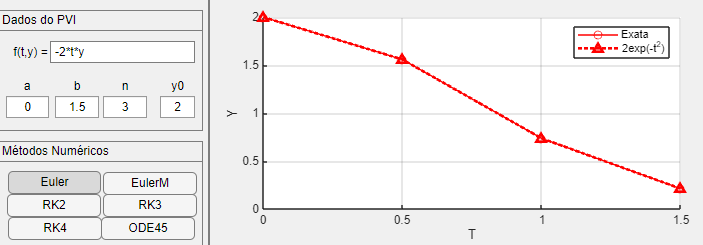
\includegraphics[width=0.9\textwidth]{Fotos/1farol3a}
    \caption{Resolução do Exercício 3.a}
    \label{fig:1farol3a}
\end{figure}

\begin{figure}[H]
    \centering
    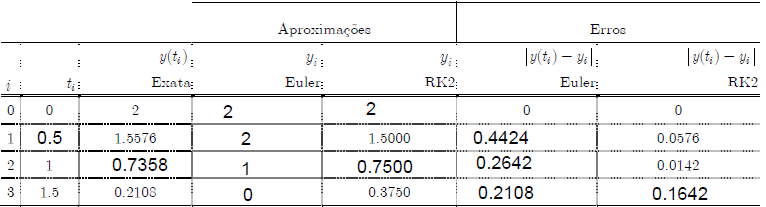
\includegraphics[width=0.9\textwidth]{Fotos/1farol3b0}
    \caption{Resolução do Exercício 3.b - Parte 0}
    \label{fig:1farol3b0}
\end{figure}

\begin{figure}[H]
    \centering
    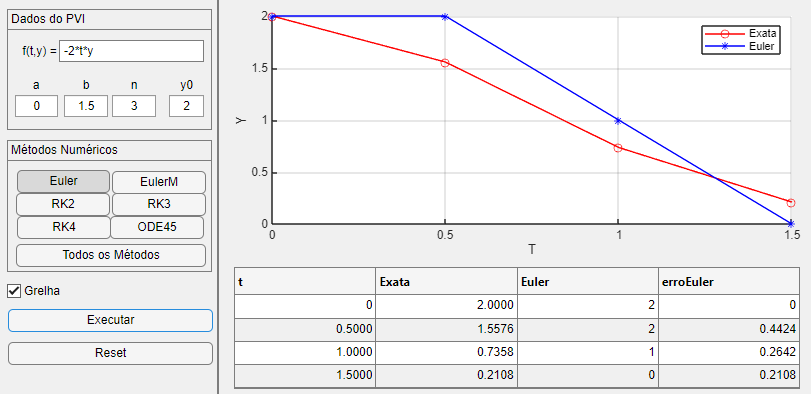
\includegraphics[width=0.9\textwidth]{Fotos/1farol3b1}
    \caption{Resolução do Exercício 3.b - Parte 1}
    \label{fig:1farol3b1}
\end{figure}

\begin{figure}[H]
    \centering
    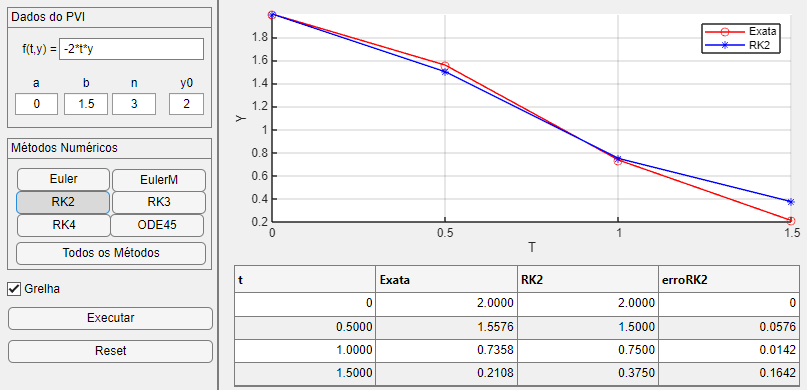
\includegraphics[width=0.9\textwidth]{Fotos/1farol3b2}
    \caption{Resolução do Exercício 3.b - Parte 2}
    \label{fig:1farol3b2}
\end{figure}

\begin{figure}[H]
    \centering
    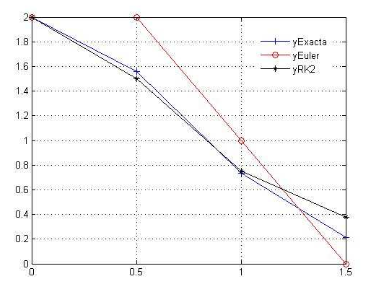
\includegraphics[width=0.9\textwidth]{Fotos/1farol3c}
    \caption{Resolução do Exercício 3.c}
    \label{fig:1farol3c}
\end{figure}

\begin{figure}[H]
    \centering
    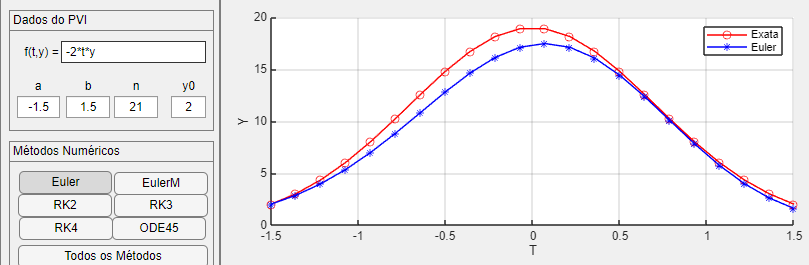
\includegraphics[width=0.9\textwidth]{Fotos/1farol3d}
    \caption{Resolução do Exercício 3.d}
    \label{fig:1farol3d}
\end{figure}

\begin{figure}[H]
    \centering
    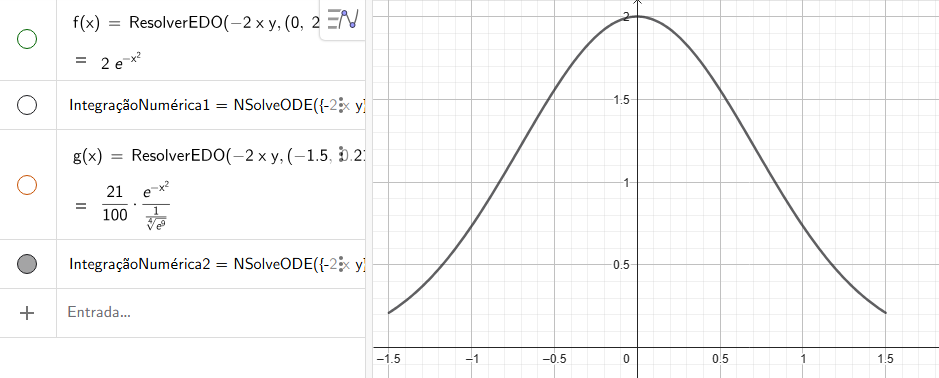
\includegraphics[width=0.9\textwidth]{Fotos/1farol3e}
    \caption{Resolução do Exercício 3.e}
    \label{fig:1farol3e}
\end{figure}

% Problemas de aplicação do livro

\section*{Problemas de Aplicação - Parte 2}

\begin{figure}[H]
    \centering
    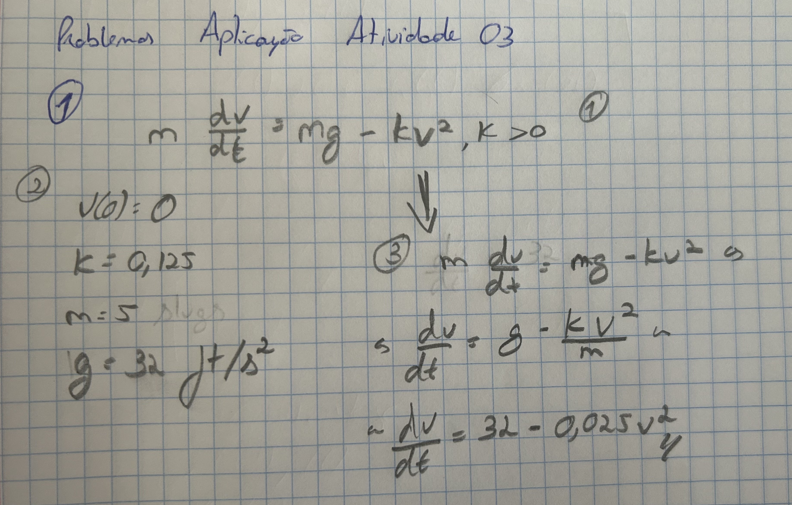
\includegraphics[width=0.9\textwidth]{Fotos/2app1a}
    \caption{Resolução do Problema do Livro 1a}
    \label{fig:2app1a}
\end{figure}

\begin{figure}[H]
    \centering
    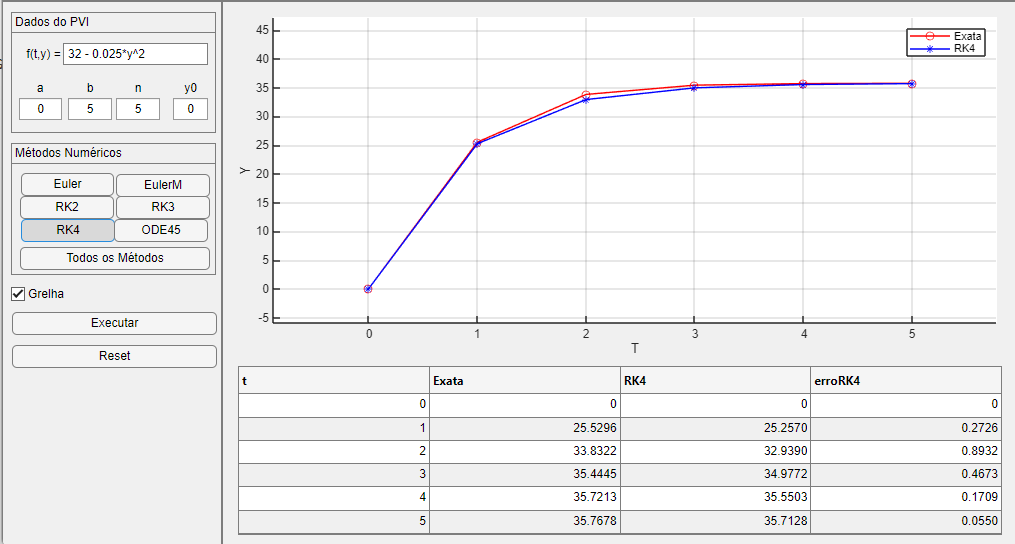
\includegraphics[width=0.9\textwidth]{Fotos/2app1b}
    \caption{Resolução do Problema do Livro 1b}
    \label{fig:2app1b}
\end{figure}

\begin{figure}[H]
    \centering
    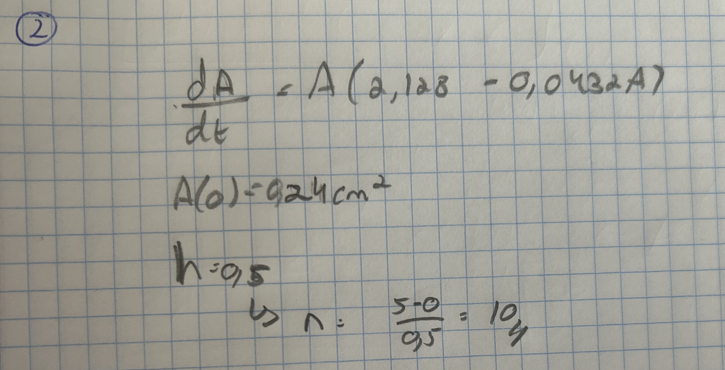
\includegraphics[width=0.9\textwidth]{Fotos/2app2a}
    \caption{Resolução do Problema do Livro 2a}
    \label{fig:2app2a}
\end{figure}

\begin{figure}[H]
    \centering
    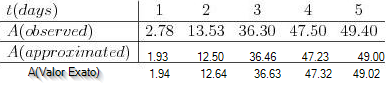
\includegraphics[width=0.9\textwidth]{Fotos/2app2b}
    \caption{Resolução do Problema do Livro 2b}
    \label{fig:2app2b}
\end{figure}

\begin{figure}[H]
    \centering
    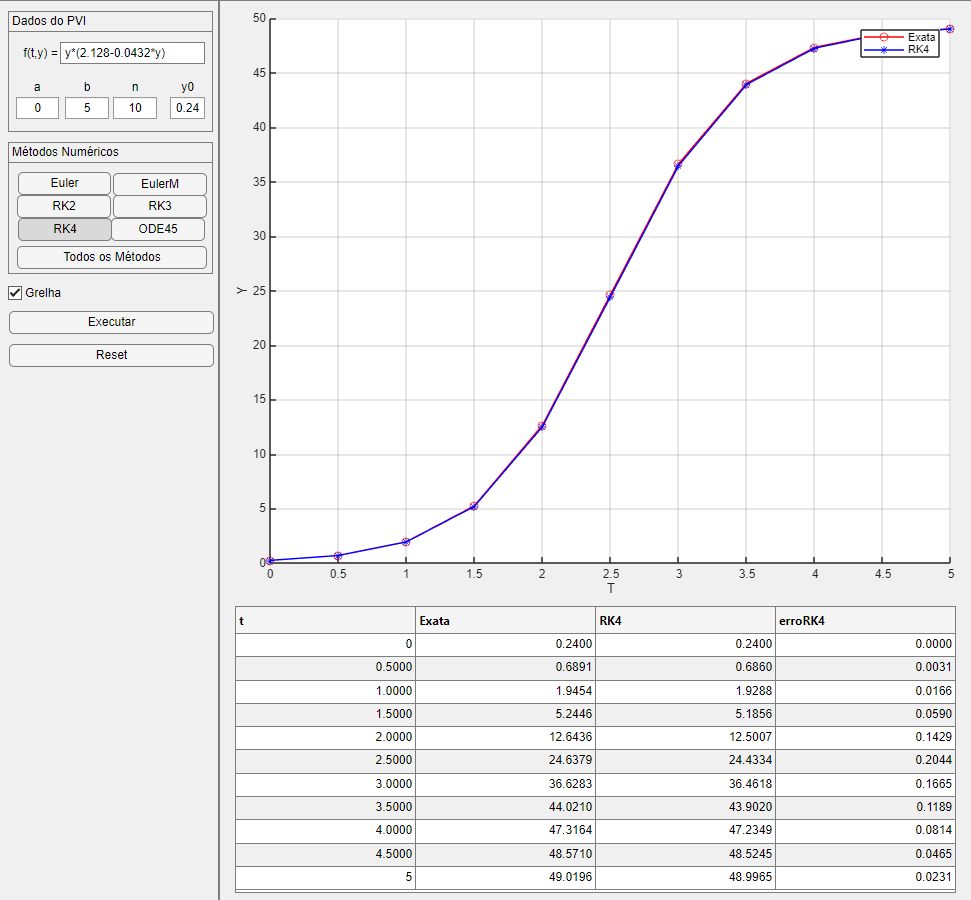
\includegraphics[width=0.9\textwidth]{Fotos/2app2c}
    \caption{Resolução do Problema do Livro 2c}
    \label{fig:2app2c}
\end{figure}

% Exercícios extra Farol

\section*{Exercícios Adicionais - Farol}

\begin{figure}[H]
    \centering
    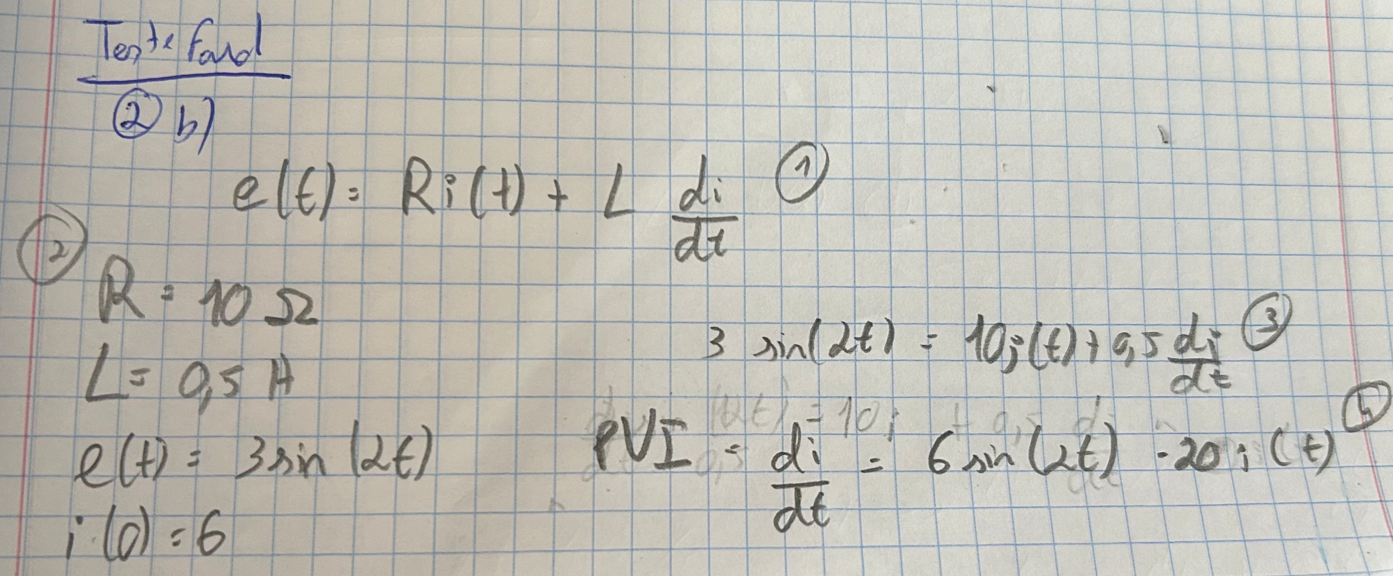
\includegraphics[width=0.9\textwidth]{Fotos/3farol1}
    \caption{Resolução do Exercício Farol Extra 1}
    \label{fig:3farol1}
\end{figure}

\begin{figure}[H]
    \centering
    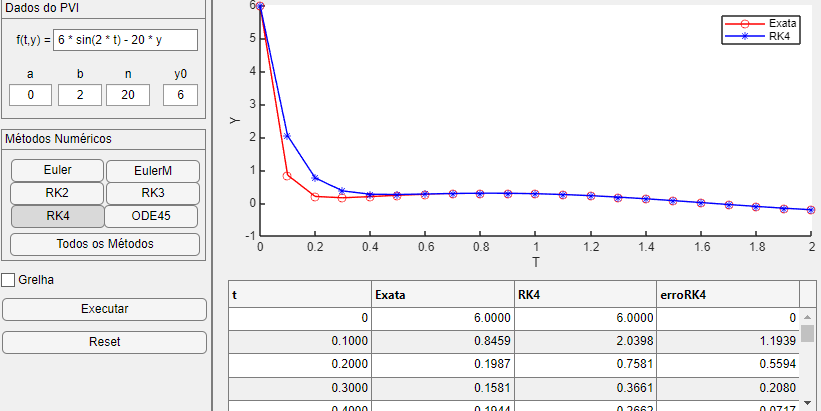
\includegraphics[width=0.9\textwidth]{Fotos/3farol2}
    \caption{Resolução do Exercício Farol Extra 2}
    \label{fig:3farol2}
\end{figure}

\begin{figure}[H]
    \centering
    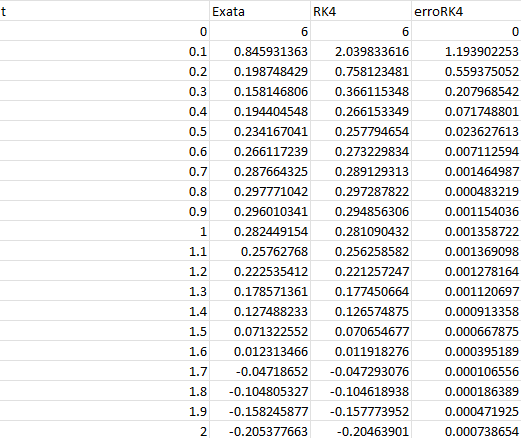
\includegraphics[width=0.9\textwidth]{Fotos/3farol3}
    \caption{Resolução do Exercício Farol Extra 3}
    \label{fig:3farol3}
\end{figure}


% Capítulo final
% Conclusão

% Conclusão
%--------------------------------------
\chapter{Conclusão}

A realização desta atividade permitiu aprofundar os conhecimentos sobre métodos numéricos para a resolução de Equações Diferenciais Ordinárias (EDO), com especial foco nos métodos de Euler, Euler melhorado, Runge-Kutta de ordens 2, 3 e 4, e o método \texttt{ode45} do \textsc{Matlab}.

Foi possível compreender não só a fundamentação teórica destes métodos, mas também as suas implementações práticas, as diferenças em termos de precisão, estabilidade e custo computacional, bem como as situações em que cada um se revela mais vantajoso. 

Através da comparação entre os resultados obtidos por diferentes métodos, ficou evidente a importância de se considerar o equilíbrio entre a complexidade do método e a precisão desejada, bem como o controlo do erro associado à discretização.

Conclui-se que os métodos de Runge-Kutta, em especial o de quarta ordem e o método \texttt{ode45}, se destacam pela sua elevada precisão em problemas com soluções suaves, sendo adequados para a maioria das aplicações práticas. No entanto, métodos mais simples como o de Euler continuam a ser úteis em contextos onde a simplicidade e o baixo custo computacional são prioritários.

Em suma, esta atividade contribuiu significativamente para a consolidação de competências na área da análise numérica, nomeadamente na aplicação prática de técnicas fundamentais para a simulação de sistemas dinâmicos descritos por EDOs.


\nocite{*}
\newpage

% Referências bibliográficas
\phantomsection
\addcontentsline{toc}{chapter}{Refer\^{e}ncias bibliogr\'{a}ficas}
\renewcommand{\bibname}{Refer\^{e}ncias bibliogr\'{a}ficas}

%-------------------
% Obs#3
% Descomentar uma das seguintes linhas, em alternativa, 
% consoante o estilo pretendido para as referências bibliográficas
\bibliographystyle{IEEEtran} % formatação segundo IEEE 
%\bibliographystyle{apacite} % formatação segundo APA 
%-------------------
\bibliography{bibliografia}

\newpage

% Anexos
%\phantomsection
%\addcontentsline{toc}{chapter}{Anexos}
%\chapter*{Anexos}

%\newpage

% Anexo A
%--------------------------------------
% Obs#4
% Definir o título do anexo A
%\newcommand{\tituloanexoA}{Título do Anexo A}
%--------------------------------------
%\phantomsection
%\addcontentsline{toc}{section}{Anexo A - \tituloanexoA}
%
% Anexo
%--------------------------------------
\vspace*{45pt}
% Título do anexo A (\tituloanexoA) definido no ficheiro main
\section*{Anexo A - \tituloanexoA}


\amostradetexto



%\newpage

% Anexo B
%--------------------------------------
% Obs#5
% Definir o título do anexo B
%\newcommand{\tituloanexoB}{Título do Anexo B}
%--------------------------------------
%\phantomsection
%\addcontentsline{toc}{section}{Anexo B - \tituloanexoB}
%
% Anexo
%--------------------------------------
\vspace*{45pt}
% Título do anexo B (\tituloanexoB) definido no ficheiro main
\section*{Anexo B - \tituloanexoB}


\amostradetexto



%\newpage

\thispagestyle{empty}

% Última página

% Última página
%--------------------------------------

\pagecolor{IsecVermelho}

\mbox{}

\vfill

\begin{center}

\includegraphics[scale=0.3]{Setup/isec-logo}
\end{center}

\newpage

\pagecolor{white}



\end{document}

